\documentclass[a4paper]{article}
\usepackage[margin=1cm]{geometry}
\usepackage{amsmath, amssymb}
\usepackage{graphicx}
\usepackage{tikz}
\usetikzlibrary{arrows.meta}
\pagestyle{empty}

\definecolor{c0}{HTML}{E53935}
\definecolor{c1}{HTML}{1E88E5}
\definecolor{c2}{HTML}{43A047}
\definecolor{c3}{HTML}{FB8C00}
\definecolor{c4}{HTML}{8E24AA}
\definecolor{c5}{HTML}{00ACC1}
\definecolor{c6}{HTML}{F4511E}
\definecolor{c7}{HTML}{3949AB}
\definecolor{c8}{HTML}{7CB342}
\definecolor{c9}{HTML}{C2185B}
\definecolor{c10}{HTML}{FF7043}
\definecolor{c11}{HTML}{26A69A}
\definecolor{c12}{HTML}{5C6BC0}
\definecolor{c13}{HTML}{FFCA28}
\definecolor{c14}{HTML}{AB47BC}

\begin{document}

\begin{center}
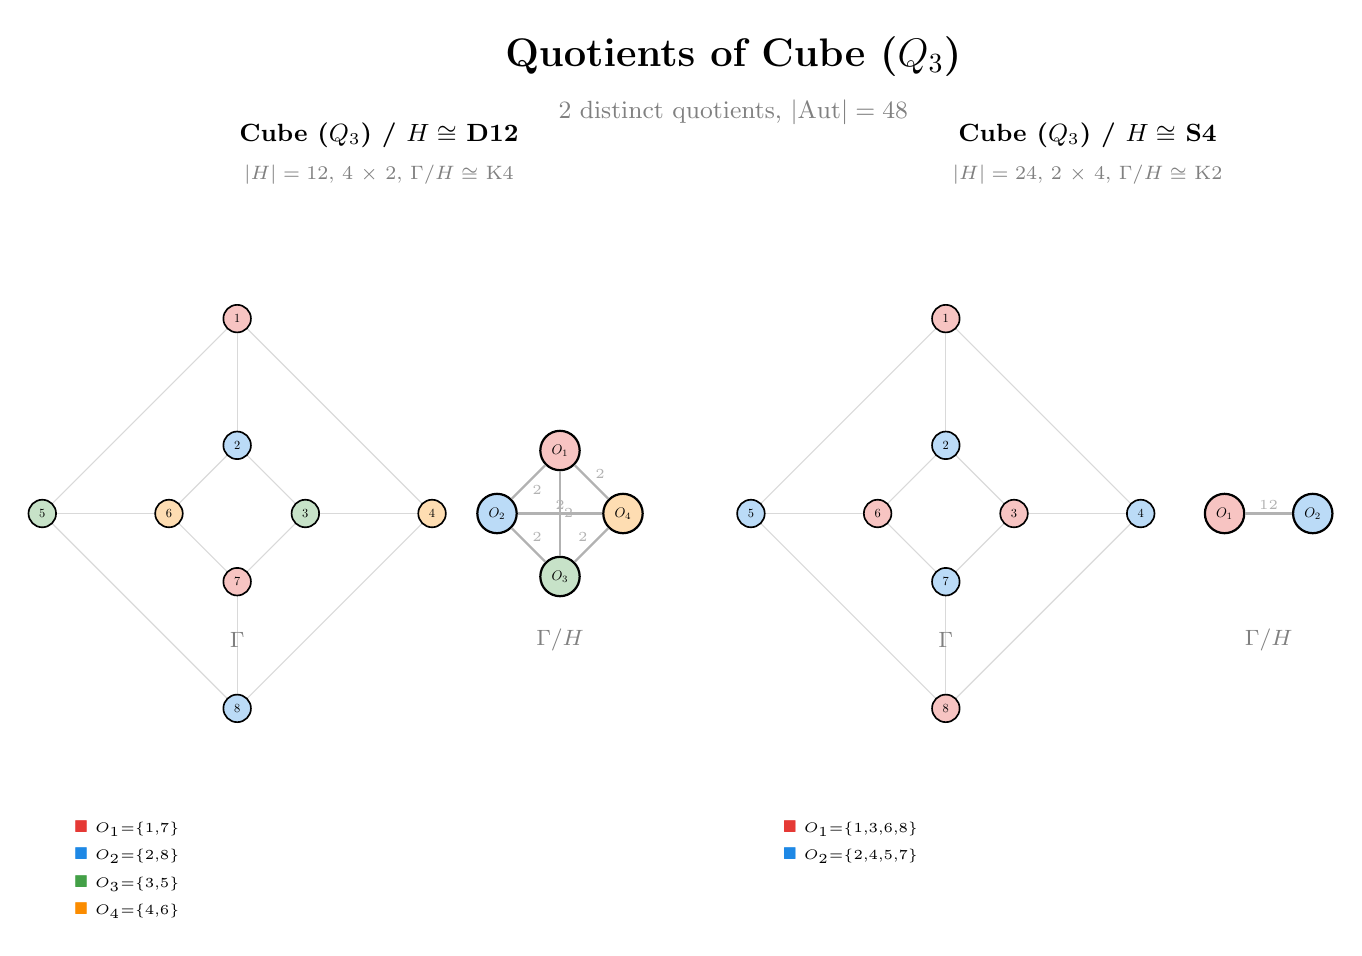
\begin{tikzpicture}[
  ov/.style={circle, draw, semithick, minimum size=3.5mm, inner sep=0pt},
  ovs/.style={circle, draw, thin, minimum size=1.8mm, inner sep=0pt},
  qv/.style={circle, draw, thick, minimum size=5mm, inner sep=0pt},
  cardtitle/.style={font=\small\bfseries},
  cardsub/.style={font=\scriptsize, text=gray},
  glabel/.style={font=\footnotesize, text=gray},
]
\node[font=\Large\bfseries] at (0, 11.5) {Quotients of Cube ($Q_3$)};
\node[font=\small, text=gray] at (0, 10.8) {2 distinct quotients, $|\mathrm{Aut}|=48$};

% Card 1: H=D12
\node[cardtitle] at (-4.50,10.50) {Cube ($Q_3$) / $H \cong$ D12};
\node[cardsub] at (-4.50,10.00) {$|H|=12$, 4 $\times$ 2, $\Gamma/H \cong$ K4};
\draw[gray!30, thin] (-6.300,8.175) -- (-6.300,6.566);
\draw[gray!30, thin] (-6.300,8.175) -- (-3.825,5.700);
\draw[gray!30, thin] (-6.300,8.175) -- (-8.775,5.700);
\draw[gray!30, thin] (-6.300,6.566) -- (-5.434,5.700);
\draw[gray!30, thin] (-6.300,6.566) -- (-7.166,5.700);
\draw[gray!30, thin] (-5.434,5.700) -- (-3.825,5.700);
\draw[gray!30, thin] (-5.434,5.700) -- (-6.300,4.834);
\draw[gray!30, thin] (-3.825,5.700) -- (-6.300,3.225);
\draw[gray!30, thin] (-8.775,5.700) -- (-7.166,5.700);
\draw[gray!30, thin] (-8.775,5.700) -- (-6.300,3.225);
\draw[gray!30, thin] (-7.166,5.700) -- (-6.300,4.834);
\draw[gray!30, thin] (-6.300,4.834) -- (-6.300,3.225);
\node[ov, fill=c0!30] at (-6.300,8.175) {\scalebox{0.45}{1}};
\node[ov, fill=c1!30] at (-6.300,6.566) {\scalebox{0.45}{2}};
\node[ov, fill=c2!30] at (-5.434,5.700) {\scalebox{0.45}{3}};
\node[ov, fill=c3!30] at (-3.825,5.700) {\scalebox{0.45}{4}};
\node[ov, fill=c2!30] at (-8.775,5.700) {\scalebox{0.45}{5}};
\node[ov, fill=c3!30] at (-7.166,5.700) {\scalebox{0.45}{6}};
\node[ov, fill=c0!30] at (-6.300,4.834) {\scalebox{0.45}{7}};
\node[ov, fill=c1!30] at (-6.300,3.225) {\scalebox{0.45}{8}};
\node[glabel] at (-6.30,4.10) {$\Gamma$};
\node[qv, fill=c0!30] (c0o0) at (-2.200,6.500) {\scalebox{0.5}{$O_{1}$}};
\node[qv, fill=c1!30] (c0o1) at (-3.000,5.700) {\scalebox{0.5}{$O_{2}$}};
\node[qv, fill=c2!30] (c0o2) at (-2.200,4.900) {\scalebox{0.5}{$O_{3}$}};
\node[qv, fill=c3!30] (c0o3) at (-1.400,5.700) {\scalebox{0.5}{$O_{4}$}};
\draw[gray!60, thick] (c0o0) -- node[font=\tiny, auto, inner sep=1pt] {2} (c0o1);
\draw[gray!60, thick] (c0o0) -- node[font=\tiny, auto, inner sep=1pt] {2} (c0o2);
\draw[gray!60, thick] (c0o0) -- node[font=\tiny, auto, inner sep=1pt] {2} (c0o3);
\draw[gray!60, thick] (c0o1) -- node[font=\tiny, auto, inner sep=1pt] {2} (c0o2);
\draw[gray!60, thick] (c0o1) -- node[font=\tiny, auto, inner sep=1pt] {2} (c0o3);
\draw[gray!60, thick] (c0o2) -- node[font=\tiny, auto, inner sep=1pt] {2} (c0o3);
\node[glabel] at (-2.20,4.10) {$\Gamma/H$};
\node[anchor=west, font=\tiny] at (-8.50,1.70) {\textcolor{c0}{$\blacksquare$} $O_{1}$=\{1,7\}};
\node[anchor=west, font=\tiny] at (-8.50,1.35) {\textcolor{c1}{$\blacksquare$} $O_{2}$=\{2,8\}};
\node[anchor=west, font=\tiny] at (-8.50,1.00) {\textcolor{c2}{$\blacksquare$} $O_{3}$=\{3,5\}};
\node[anchor=west, font=\tiny] at (-8.50,0.65) {\textcolor{c3}{$\blacksquare$} $O_{4}$=\{4,6\}};

% Card 2: H=S4
\node[cardtitle] at (4.50,10.50) {Cube ($Q_3$) / $H \cong$ S4};
\node[cardsub] at (4.50,10.00) {$|H|=24$, 2 $\times$ 4, $\Gamma/H \cong$ K2};
\draw[gray!30, thin] (2.700,8.175) -- (2.700,6.566);
\draw[gray!30, thin] (2.700,8.175) -- (5.175,5.700);
\draw[gray!30, thin] (2.700,8.175) -- (0.225,5.700);
\draw[gray!30, thin] (2.700,6.566) -- (3.566,5.700);
\draw[gray!30, thin] (2.700,6.566) -- (1.834,5.700);
\draw[gray!30, thin] (3.566,5.700) -- (5.175,5.700);
\draw[gray!30, thin] (3.566,5.700) -- (2.700,4.834);
\draw[gray!30, thin] (5.175,5.700) -- (2.700,3.225);
\draw[gray!30, thin] (0.225,5.700) -- (1.834,5.700);
\draw[gray!30, thin] (0.225,5.700) -- (2.700,3.225);
\draw[gray!30, thin] (1.834,5.700) -- (2.700,4.834);
\draw[gray!30, thin] (2.700,4.834) -- (2.700,3.225);
\node[ov, fill=c0!30] at (2.700,8.175) {\scalebox{0.45}{1}};
\node[ov, fill=c1!30] at (2.700,6.566) {\scalebox{0.45}{2}};
\node[ov, fill=c0!30] at (3.566,5.700) {\scalebox{0.45}{3}};
\node[ov, fill=c1!30] at (5.175,5.700) {\scalebox{0.45}{4}};
\node[ov, fill=c1!30] at (0.225,5.700) {\scalebox{0.45}{5}};
\node[ov, fill=c0!30] at (1.834,5.700) {\scalebox{0.45}{6}};
\node[ov, fill=c1!30] at (2.700,4.834) {\scalebox{0.45}{7}};
\node[ov, fill=c0!30] at (2.700,3.225) {\scalebox{0.45}{8}};
\node[glabel] at (2.70,4.10) {$\Gamma$};
\node[qv, fill=c0!30] (c1o0) at (6.240,5.700) {\scalebox{0.5}{$O_{1}$}};
\node[qv, fill=c1!30] (c1o1) at (7.360,5.700) {\scalebox{0.5}{$O_{2}$}};
\draw[gray!60, thick] (c1o0) -- node[font=\tiny, auto, inner sep=1pt] {12} (c1o1);
\node[glabel] at (6.80,4.10) {$\Gamma/H$};
\node[anchor=west, font=\tiny] at (0.50,1.70) {\textcolor{c0}{$\blacksquare$} $O_{1}$=\{1,3,6,8\}};
\node[anchor=west, font=\tiny] at (0.50,1.35) {\textcolor{c1}{$\blacksquare$} $O_{2}$=\{2,4,5,7\}};
\end{tikzpicture}
\end{center}

\end{document}